\documentclass[12pt,a4paper]{ctexart}
\usepackage[margin=2.2cm]{geometry}
\usepackage{graphicx}
\usepackage{booktabs}
\usepackage{amsmath}
\usepackage{float}
\usepackage{hyperref}
\usepackage{xcolor}
\usepackage{listings}
\usepackage{amssymb}

\lstset{
  language=Python,
  basicstyle=\ttfamily\small,
  keywordstyle=\color{blue!70!black},
  commentstyle=\color{green!40!black},
  stringstyle=\color{orange!60!black},
  showstringspaces=false,
  breaklines=true,
  frame=single,
  tabsize=2
}

\newcommand{\reporttitle}{Project 8：摄像机标定实验报告}
\newcommand{\authname}{姓名}
\newcommand{\authid}{学号}
\newcommand{\class}{班级}

\title{\reporttitle}
\author{\authname：\underline{李祥熙} \quad \authid：\underline{2234412799} \quad \class：\underline{计算机2301}}
\date{}

\begin{document}
\maketitle
\tableofcontents
\newpage

% =====================================================================
\section{实验目的}
% =====================================================================

\begin{itemize}
  \item \textbf{理解摄像机标定原理}：掌握张正友标定法（Zhang's method）的基本理论，了解内参矩阵、畸变系数与外参的含义。
  \item \textbf{熟悉 OpenCV 标定流程}：使用 OpenCV 提供的 \texttt{calibrateCamera} 函数，对真实手机镜头进行标定。
  \item \textbf{分析镜头畸变特性}：通过对标定结果的分析，理解径向畸变与切向畸变在实际镜头中的表现。
  \item \textbf{实现畸变矫正}：利用标定得到的内参和畸变系数，对真实图像进行畸变矫正，验证标定结果的有效性。
\end{itemize}

% =====================================================================
\section{实验环境}
% =====================================================================

\begin{itemize}
  \item 操作系统：Linux（Arch Linux）
  \item 编程语言：Python 3
  \item 主要工具：Jupyter Notebook、OpenCV、NumPy
  \item 拍摄设备：% TODO: 填写手机型号和镜头信息，例如"小米14 主摄（IMX989，1英寸，f/1.6）"
\end{itemize}

% =====================================================================
\section{实验过程}
% =====================================================================

基本实验过程如下：

\begin{enumerate}
  \item 利用 Python 脚本（\texttt{checkerboard.py}）生成棋盘格图像并打印；
  \item 拍摄若干张不同角度和距离的棋盘格图像，关闭手机自带的镜头矫正功能；
  \item 运行 \texttt{calibration.ipynb} 进行角点检测和摄像机标定，获得内参、畸变系数和外参；
  \item 利用内参和畸变系数对另一张图像进行畸变矫正。
\end{enumerate}

% =====================================================================
\section{摄像机标定理论}
% =====================================================================

本实验使用 OpenCV 实现的张正友标定法。OpenCV 中的畸变模型包含径向畸变和切向畸变两部分。

\subsection{径向畸变}

径向畸变由镜头形状引起，其模型为

\begin{equation}
  x_\text{distorted} = x\bigl(1 + k_1 r^2 + k_2 r^4 + k_3 r^6\bigr), \quad
  y_\text{distorted} = y\bigl(1 + k_1 r^2 + k_2 r^4 + k_3 r^6\bigr)
\end{equation}

其中 $r^2 = x^2 + y^2$，$(x, y)$ 为归一化图像坐标，$k_1, k_2, k_3$ 为径向畸变系数。

\subsection{切向畸变}

切向畸变由镜头与成像平面不完全平行引起，其模型为

\begin{equation}
  x_\text{distorted} = x + \bigl[2p_1 xy + p_2(r^2 + 2x^2)\bigr], \quad
  y_\text{distorted} = y + \bigl[p_1(r^2 + 2y^2) + 2p_2 xy\bigr]
\end{equation}

其中 $p_1, p_2$ 为切向畸变系数。综合两种畸变，最终的畸变系数为五元组

\begin{equation}
  \text{Distortion coefficients} = \begin{pmatrix} k_1 & k_2 & p_1 & p_2 & k_3 \end{pmatrix}
\end{equation}

% =====================================================================
\section{相机标定结果}
% =====================================================================

\subsection{角点检测}

对每张棋盘格图像进行 9×6 内角点检测，结果如图 \ref{fig:corners} 所示。

\begin{figure}[H]
  \centering
  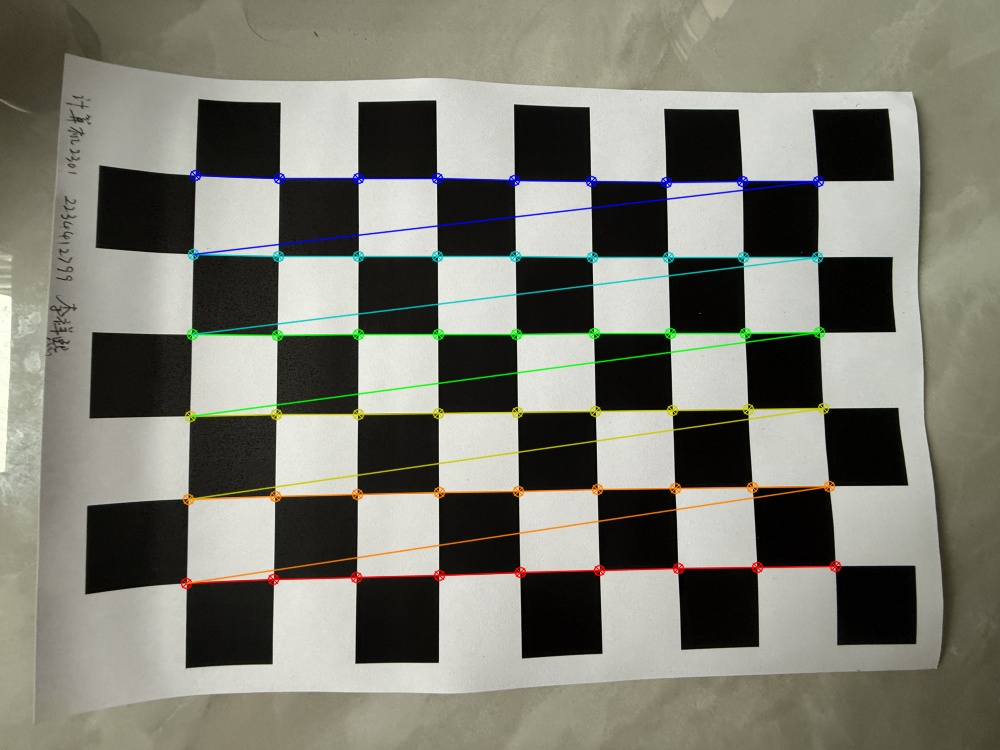
\includegraphics[width=0.30\textwidth]{../corner/0.jpg}
  
\includegraphics[width=0.30\textwidth]{../corner/1.jpg}
  
\includegraphics[width=0.30\textwidth]{../corner/2.jpg}\\[4pt]
  
\includegraphics[width=0.30\textwidth]{../corner/3.jpg}
  
\includegraphics[width=0.30\textwidth]{../corner/4.jpg}
  
\includegraphics[width=0.30\textwidth]{../corner/5.jpg}
  \caption{各标定图像的角点检测结果}
  \label{fig:corners}
\end{figure}

\subsection{内参矩阵}

标定得到的相机内参矩阵 $K$ 如下：

\begin{equation}
  K = \begin{pmatrix}
    733.39419537 & 0            & 503.82907973 \\
    0            & 732.11725156 & 369.89539954 \\
    0            & 0            & 1
  \end{pmatrix}
\end{equation}

\subsection{畸变系数}

\begin{table}[H]
  \centering
  \caption{畸变系数}
  \begin{tabular}{ccccc}
    \toprule
    $k_1$ & $k_2$ & $p_1$ & $p_2$ & $k_3$ \\
    \midrule
    $0.24604382$ & $-1.01102813$ & $-0.00450469$ & $0.00264820$ & $1.64885357$ \\
    \bottomrule
  \end{tabular}
\end{table}

\subsection{外参（第一张图像）}

对应第一张标定图像的旋转向量 $r_1$ 和平移向量 $t_1$ 如下：

\begin{equation}
  r_1 = \begin{pmatrix}
    -0.05866420 \\ 0.94653745 \\ 2.97498748
  \end{pmatrix}, \quad
  t_1 = \begin{pmatrix}
    4.28616412 \\ 1.85310577 \\ 10.23931967
  \end{pmatrix}
\end{equation}

其中旋转向量为 Rodrigues 形式，可通过 \texttt{cv2.Rodrigues()} 转换为旋转矩阵。

% =====================================================================
\section{畸变矫正结果}
% =====================================================================

使用一张另拍摄的未矫正图像（图 \ref{fig:sample}），利用标定得到的内参和畸变系数进行畸变矫正。

\begin{figure}[H]
  \centering
  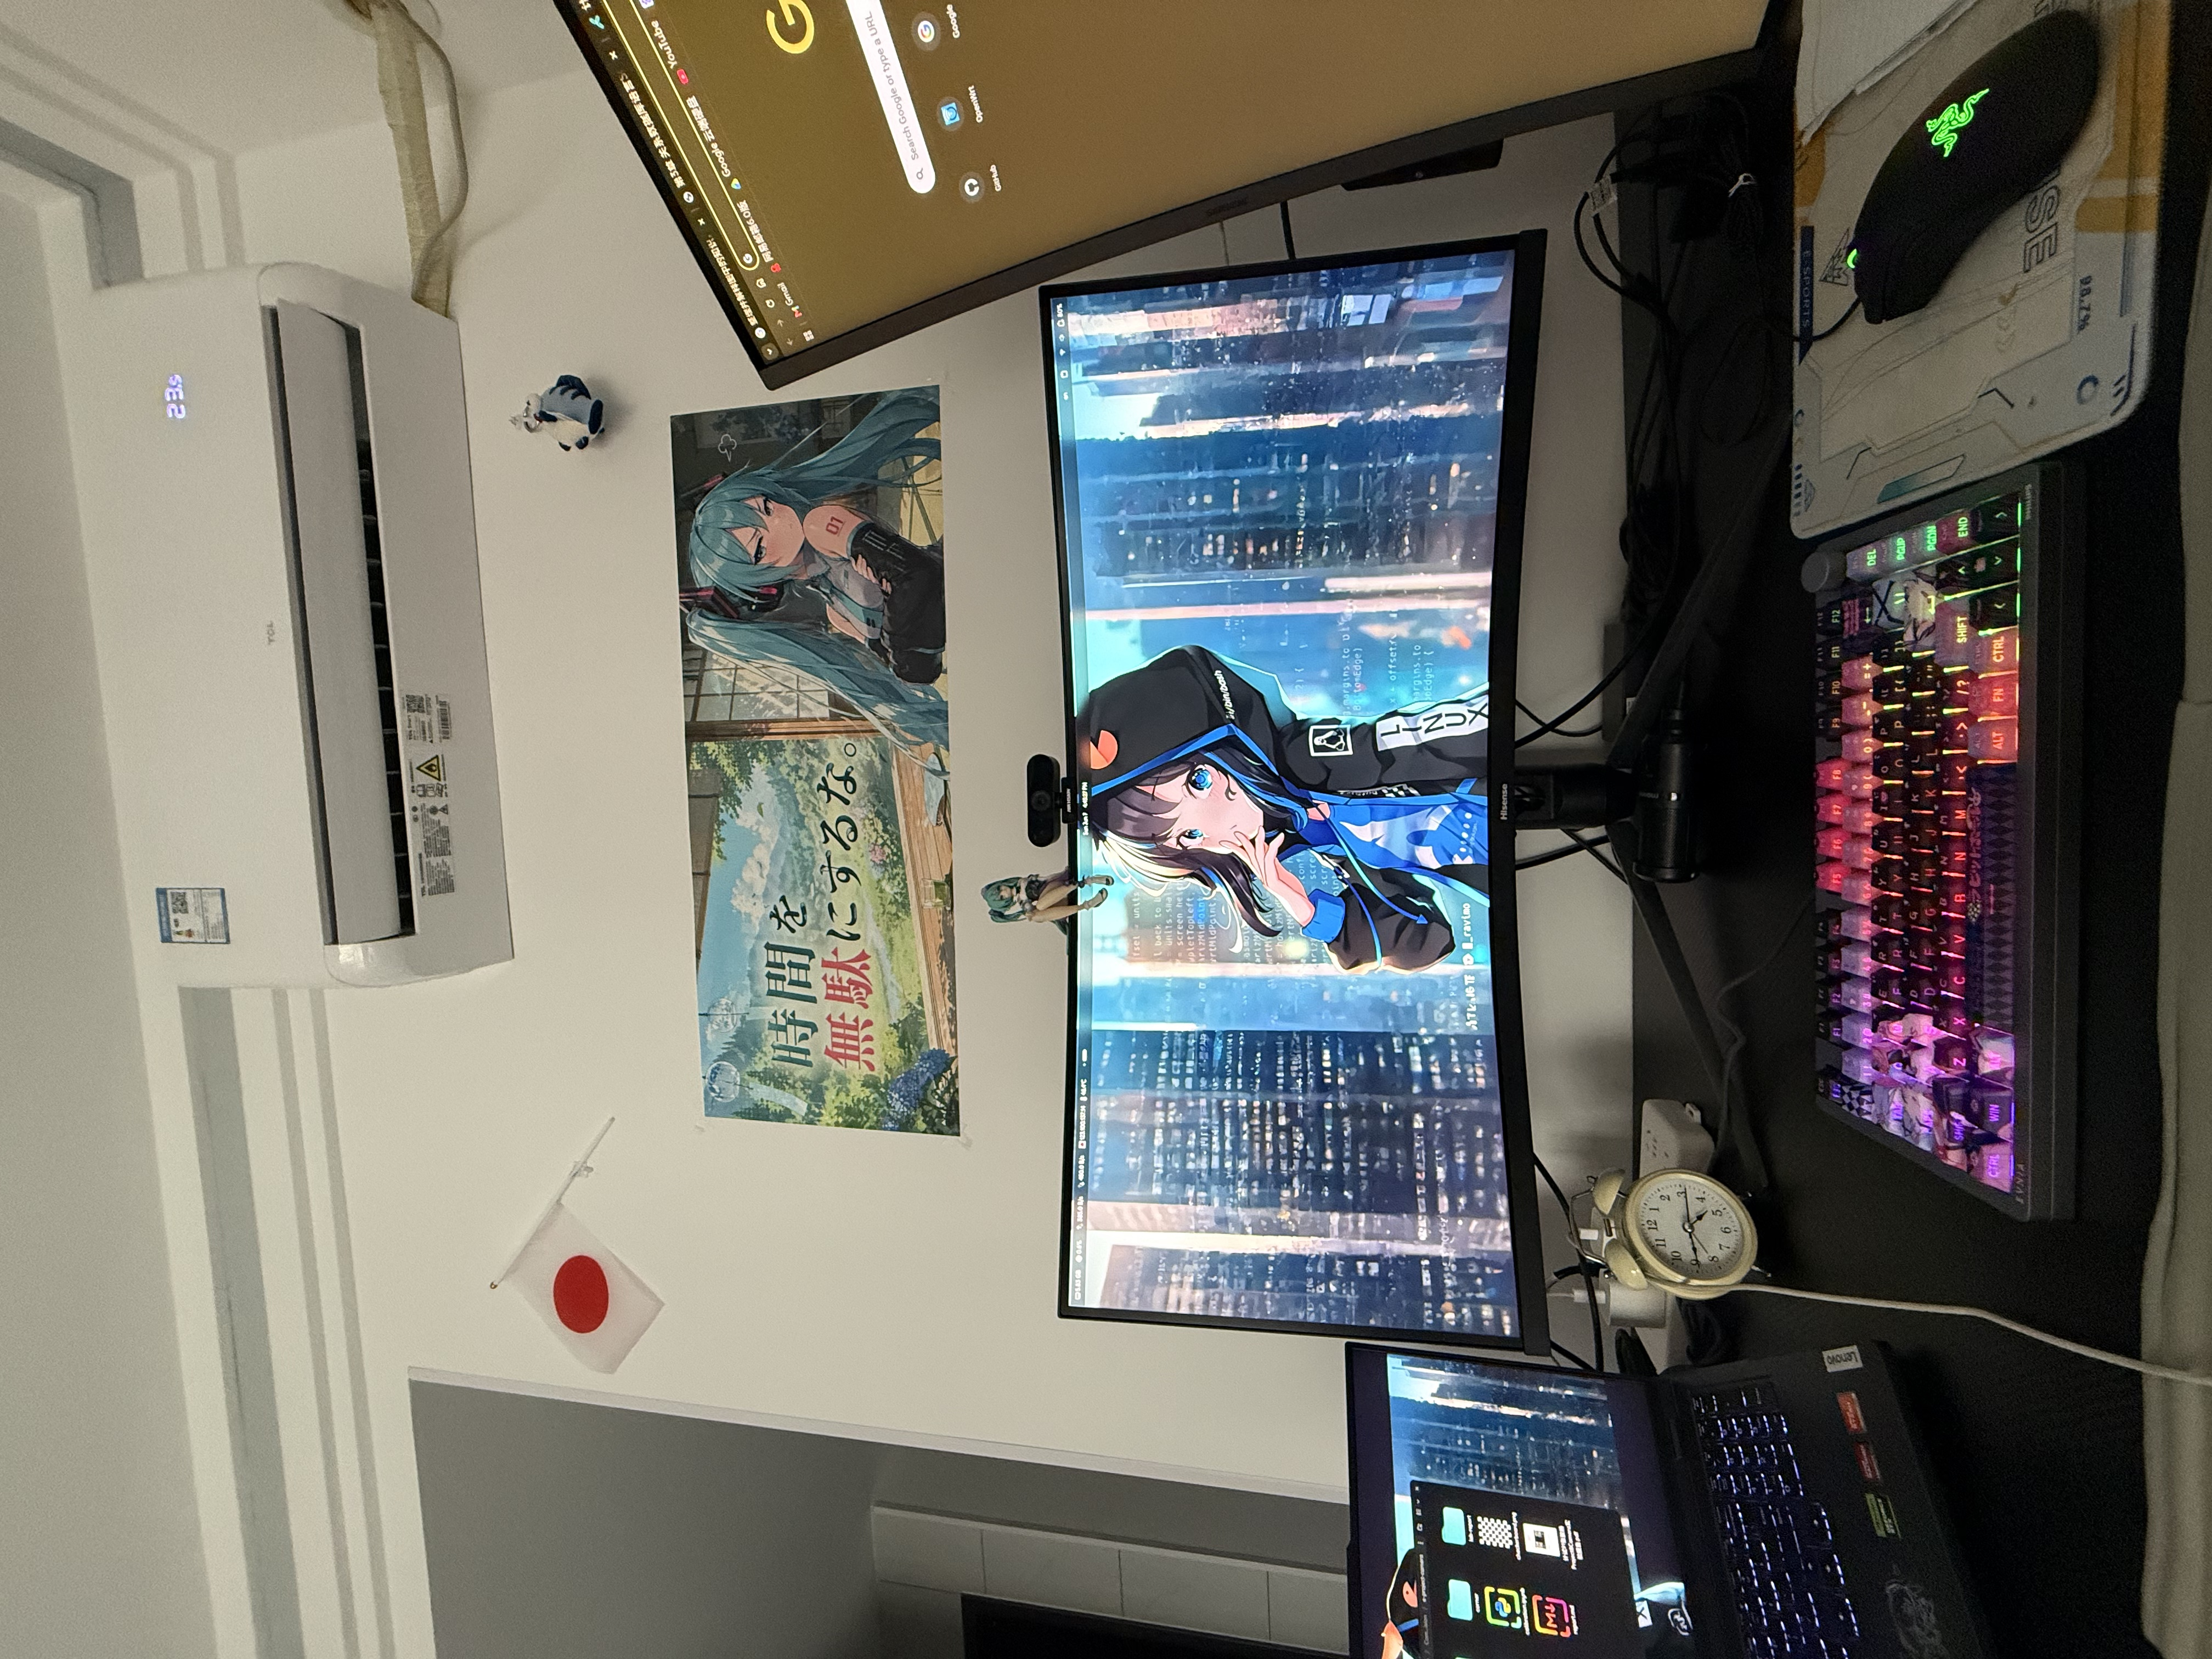
\includegraphics[width=0.55\textwidth]{../samples/sample.jpg}
  \caption{原始未矫正图像}
  \label{fig:sample}
\end{figure}

畸变矫正后（保留完整画面）的结果如图 \ref{fig:nocrop} 所示，对无效区域裁剪后的结果如图 \ref{fig:cropped} 所示。

\begin{figure}[H]
  \centering
  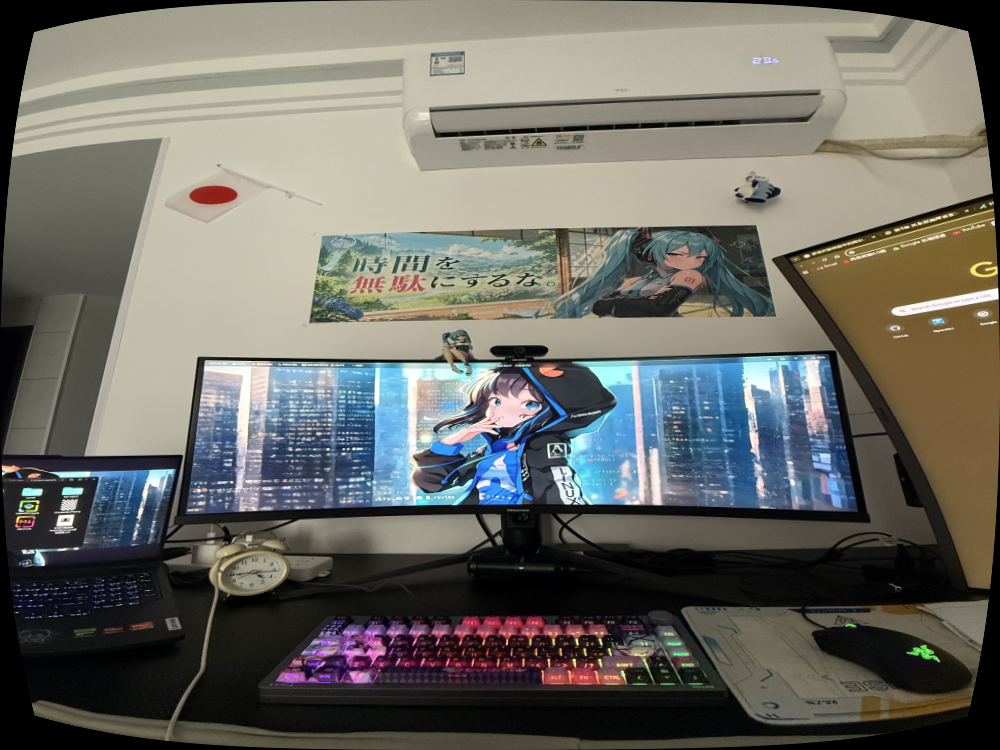
\includegraphics[width=0.55\textwidth]{../undistorted/calibresult_nocrop_0.png}
  \caption{畸变矫正后（含黑色边缘区域）}
  \label{fig:nocrop}
\end{figure}

\begin{figure}[H]
  \centering
  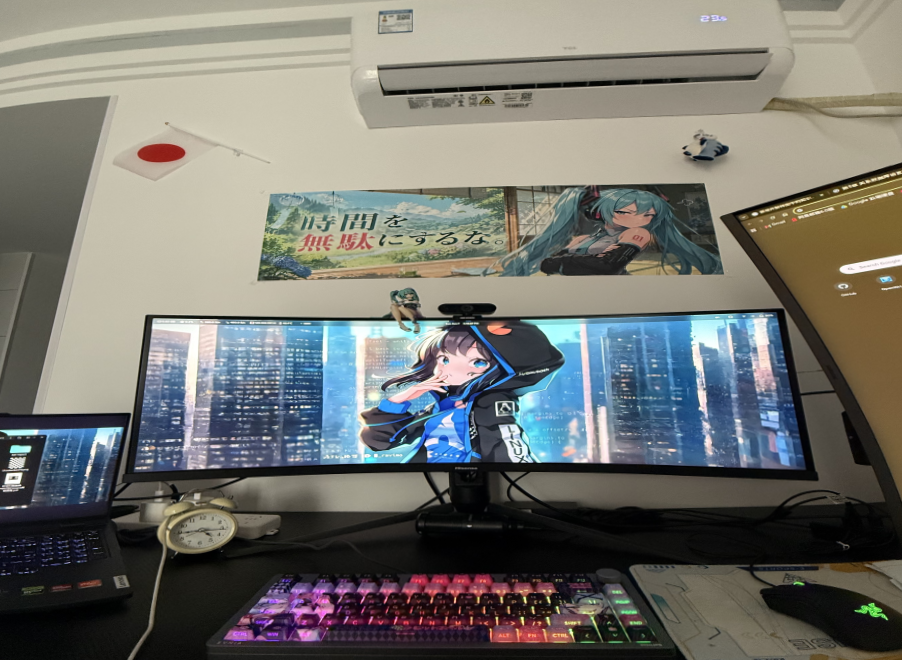
\includegraphics[width=0.55\textwidth]{../undistorted/calibresult_0.png}
  \caption{畸变矫正后（裁剪至有效区域）}
  \label{fig:cropped}
\end{figure}

% =====================================================================
\section{参考文献}
% =====================================================================

\begin{enumerate}
  \item OpenCV Camera Calibration Tutorial, \url{https://docs.opencv.org/4.x/dc/dbb/tutorial_py_calibration.html}
  \item OpenCV Rodrigues, \url{https://docs.opencv.org/4.x/d9/d0c/group__calib3d.html#ga61585db663d9da06b68e70cfbf6a1eac}
\end{enumerate}

% =====================================================================
\appendix
\section{附录：标定代码}
% =====================================================================

\subsection{生成棋盘格图像}

\begin{lstlisting}
from PIL import Image

h, hc = 2000, 10
w, wc = 1400, 7
img = Image.new("RGB", (w, h), (0, 0, 0))
pixels = img.load()
for i in range(w):
    for j in range(h):
        if ((i // (h // hc)) & 1) ^ ((j // (w // wc)) & 1):
            pixels[i, j] = (0, 0, 0)
        else:
            pixels[i, j] = (255, 255, 255)
img.save('./checkerboard.png')
\end{lstlisting}

\subsection{角点检测与摄像机标定}

\begin{lstlisting}
import cv2, numpy as np, glob

CHECKERBOARD = (9, 6)
criteria = (cv2.TERM_CRITERIA_EPS + cv2.TERM_CRITERIA_MAX_ITER, 50, 0.001)
objectp3d = np.zeros((1, CHECKERBOARD[0] * CHECKERBOARD[1], 3), np.float32)
objectp3d[0, :, :2] = np.mgrid[0:CHECKERBOARD[0], 0:CHECKERBOARD[1]].T.reshape(-1, 2)

threedpoints, twodpoints = [], []
for i, filename in enumerate(glob.glob('./checkerboards/*.jpg')):
    image = cv2.resize(cv2.imread(filename), (1000, 750))
    gray = cv2.cvtColor(image, cv2.COLOR_BGR2GRAY)
    ret, corners = cv2.findChessboardCorners(gray, CHECKERBOARD,
        cv2.CALIB_CB_ADAPTIVE_THRESH + cv2.CALIB_CB_FAST_CHECK +
        cv2.CALIB_CB_NORMALIZE_IMAGE)
    if ret:
        threedpoints.append(objectp3d)
        corners2 = cv2.cornerSubPix(gray, corners, (20, 20), (-1, -1), criteria)
        twodpoints.append(corners2)
        cv2.drawChessboardCorners(image, CHECKERBOARD, corners2, ret)
    cv2.imwrite(f'./corner/{i}.jpg', image)

ret, matrix, distortion, r_vecs, t_vecs = cv2.calibrateCamera(
    threedpoints, twodpoints, gray.shape[::-1], None, None)
print("Camera matrix:\n", matrix)
print("Distortion coefficients:\n", distortion)
\end{lstlisting}

\subsection{畸变矫正}

\begin{lstlisting}
import cv2, glob

for i, filename in enumerate(glob.glob('./samples/*.jpg')):
    img = cv2.resize(cv2.imread(filename), (1000, 750))
    h, w = img.shape[:2]
    newmtx, roi = cv2.getOptimalNewCameraMatrix(matrix, distortion, (w, h), 1, (w, h))
    dst = cv2.undistort(img, matrix, distortion, None, newmtx)
    cv2.imwrite(f'./undistorted/calibresult_nocrop_{i}.png', dst)
    x, y, w, h = roi
    cv2.imwrite(f'./undistorted/calibresult_{i}.png', dst[y:y+h, x:x+w])
\end{lstlisting}

\end{document}
